\documentclass[a4paper]{article}

\usepackage[english]{babel}
\usepackage[utf8x]{inputenc}
\usepackage{amsmath}
\usepackage{graphicx}
\usepackage[colorinlistoftodos]{todonotes}
\usepackage{enumitem}
\usepackage{verbatim} % for multiline comments

\title{System Validation: Project}
\author{J.M. Somers, C. Roest, D. van den Heuvel \& I.C.T.M Speek}

\begin{document}
\maketitle

%----------------------------------------------------------------%

\begin{comment}
  \begin{abstract}
  Your abstract.
  \end{abstract}
\end{comment}

%----------------------------------------------------------------%

\section{Introduction}
\label{sec:introduction}
% intoductie tot complexiteit brug systemen
% wat moet de safety controller kunnen
% korte volgorde van alle handelingen
% onze taken
% introductie tot parallele componenten en architectuur
% verwijzen naar wat er in elke sectie gebeurt
%
The Dutch governmental organisation Rijkswaterstaat is responsible for the core infrastructure of the Netherlands. Active components in the infrastructure such as bridges and sluices require safety control layers as indicated by safety regulations and previous experiences in designing these. These layers must ensure the absence of unsafe situations at all times. They should however not unnecessarily impact the flow of trafic in a negative way. 

In this report we will design a safety controller for a bridge system. This safety controller will either validate or reject the input from an interface controller operated by the user. To ensure no unsafe situations will ever occur, a worst case scenario in which the emergency contols are operated is assumed. The user can  control all objects as listed in Section \ref{sec:objects} in the system independently while the emergency controls are enabled. 

The model depicted in figure \ref{fig:model} displays the different components of the system. The safety controller is in charge of validation of the instuctions passed on by the interface controller. Depending on the input from a list of sensors, the safety controller can sequentially enable the pre-sign lights, the stop-sign lights, close the barrier for incoming traffic and close the barrier for outgoing traffic. If this situation is validated as safe as defined in Section \ref{sec:definitions} the safety controller will allow the motor to raise the bridge so that boats can pass. The opposite counts for lowering the bridge to let traffic pass. Within this model we assume that external features such as traffic will behave according to traffic rules and boat traffic will be accounted for by the bridge operator through the interface controller. 

For this project we will describe the global requirements of the system and indentify the relevant interactions. By grouping the objects into parallel components we will describe an architecture of the structure of the system. The global requirements can then further be translated in terms of these interactions. The system behavior can then be described and verified using mCRL2. 

In this report we will design a safety controller for a bridge system. The model of the system, its objects and concurrent definitions are introduced in Section \ref{sec:model}. Section \ref{sec:requirements} introduces the requirements. 			% introduction.tex wordt hier geimporteerd
% intoductie tot complexiteit brug systemen
% wat moet de safety controller kunnen
% onze taken
% introductie tot parallele componenten en architectuur
% verwijzen naar wat er in elke sectie gebeurt


%----------------------------------------------------------------%
\newpage
\section{The model}
\label{sec:model}
\todo{Make own images}
% Give an introduction to the situational sketch and model system
% Present the communication model
% Argument design choices

We created a model for our bridge to account for the sequenced actions necessary to open and close the bridge in a safe manner. The model and its components are displayed in figure \ref{fig:model}. 
%--------------- Image of the model------------

\begin{figure}[!h]
\centering
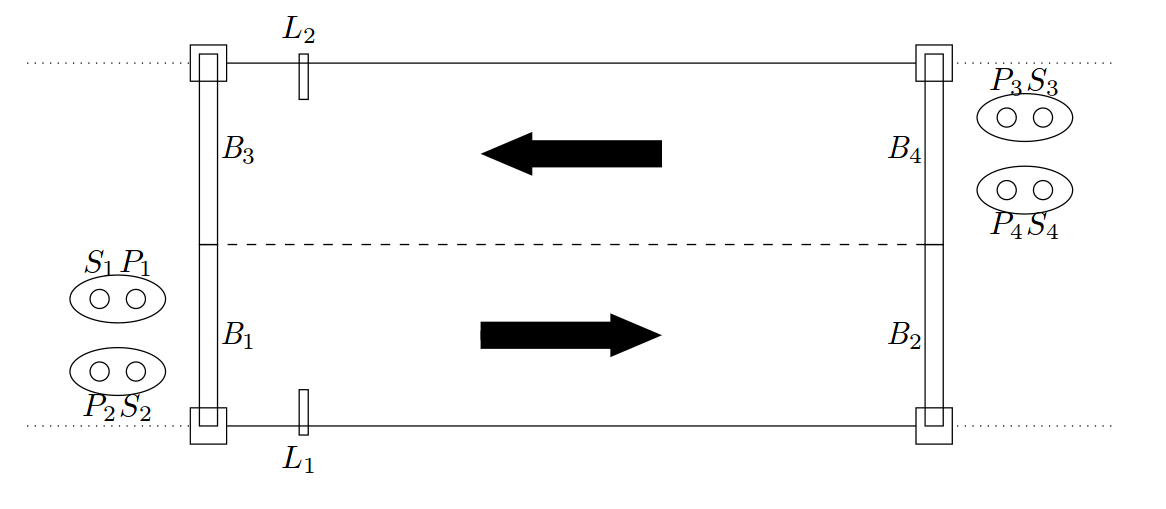
\includegraphics[width=1\textwidth]{sketch.png}
\caption{A situational sketch of the model and its components}
\label{fig:model}
\end{figure}

Our model also includes several sensors that will validate the preconditions that are required for our chain of actions. These sensors and their concurring sequence of actions are displayed in figure \ref{fig:sequence}. Using this chain of actions the global set of requirement was made. 


%--------------- Image of the sequence ------------
\begin{figure}[!h]
\centering
\includegraphics[width=0.5\textwidth]{model.pdf}
\caption{The sequence of actions in our model and the supporting sensors}
\label{fig:sequence}
\end{figure}

% Give an introduction to the situational sketch and model system
% Present the communication model
% Argument design choices

\subsection{Objects}
\label{sec:objects}
\todo{argument objects and their numbers}

\begin{enumerate}

\item{Control system} \\
The system that gives the instructions to the safety controler for "when" actions have to be done. 
\begin{itemize}
\item{User}
\item{Interface Controller} 
\end{itemize}
output: Unsafe actions to control the different elements of the bridge. \\
actions: The user (or any other system behind the interface controler) determines when different actions should take place. \\
input: status of the other subsystems. 

\item{Safety controller} \\
The system that checks if the given actions from the control system are safe according to the status of the different components. 
\begin{itemize}
\item{contains no other objects} 
\end{itemize}
output: safe actions to control the different elements of the bridge, is able to report status errors to the control system. \\
actions: Check status of different objects. \\
input: unsafe actions. 

\item{Bridge-deck system}
\begin{itemize}
\item{3 sensors: Bridge is open}
\item{3 sensors: Bridge is closed}
\item{3 sensors: Bridge locking pins state}
\item{2 locking pins}
\item{Bridge break}\item{Bridge motor. This also indicates a state \{Stopped, Moving up, moving down, broken\}}
\end{itemize}
input: action requests for opening or closing the bridge. \\
actions: control the right sequence of brigde-objects to open or close the bridge\\
output: status of different components. 

\item{Light system}
\begin{itemize}
\item{2 orange Lights for lane 1}
\item{2 orange Lights for lane 2}
\item{2 red Lights for lane 1}
\item{2 red Lights for lane 2}
\end{itemize}
input: Status request of the lights, or action request to change the status of the lights \\
actions: change the status of the lights\\
output: Status of the different lights:\{on, off, broken\}.
 

\item{barier system}
\begin{itemize}
\item{inner barier 1}
\item{outer barier 1}
\item{2 sensors for if inner barier of lane 1 is open}
\item{2 sensors for if outer barier of lane 1 is open}
\item{2 sensors for if inner barier of lane 1 is closed}
\item{2 sensors for if outer barier of lane 1 is closed}
\item{inner barier 2}
\item{outer barier 2}
\item{2 sensors for if inner barier of lane 2 is open}
\item{2 sensors for if outer barier of lane 2 is open}
\item{2 sensors for if inner barier of lane 2 is closed}
\item{2 sensors for if outer barier of lane 2 is closed}
\end{itemize}
input: actions to control the different objects of the barier system. \\
actions: change state of objects of the barier system. \\
output: status of objects of the barier system. 

%----------------------------------------------------------------%

\end{enumerate}

\subsection{Definitions}
\label{sec:definitions}

\begin{enumerate}
\item{The bridge is open if the 2 out of 3 sensors indicate that the bridge is open.}
\item{The bridge is closed if the 2 out of 3 sensors indicate that the bridge is closed.}
\item{The bridge is in undefined state when the bridge is not open and not closed.}
\item{When the input of the safety controller issues to open the bridge, the bridge is going to be opened in precise order discribed in \ref{openBridge}}
\item{When the input of the safety controller issues to open the bridge, the bridge is going to be opened in precise order discribed in \ref{closeBridge}}
\item{Traffic flow is hampered when the bridge is in a state where both cars and vessels cannot cross.}
\item{The barriers that the cars will encounter first will be called "first barriers"}
\item{The barriers that the cars will encounter last will be called "last barriers"}

\end{enumerate}



%----------------------------------------------------------------%

\section{Requirements}
\label{sec:requirements}

Case: bridge is going to be opened
\label{openBridge}
\begin{enumerate}

\item{The red lights may not go on if the yelow lights are not already on.}
\item{The barriers may not close if the red lights are not on.}
\item{\label{item:traffic}If there is traffic on the bridge, the bariers may not close.}
%\item{The bridge may not open if the barriers are not closed.}
\item{The last barriers can close if and only if the first barriers are closed.}
\item{The bridge may not open if not all barriers are closed.}
\item{The bridge may not open if the locking pins are engaged.}

\end{enumerate}


\noindent Case: bridge is going to be closed
\label{closeBridge}
\begin{enumerate}[resume]

\item{The barriers may not open if the bridge is not closed.}
\item{The red lights may not go out when the bariers are not up.}
\item{The locking pins may not engage if the bridge is not closed.}

%\item{The bridge may not close if the ship has not completely passed the bridge.}


\end{enumerate}

\noindent General Requirements

\begin{enumerate}[resume]

\item{The break must be applied if the bridge is open and is not going to close}
\item{The break must be applied if the bridge is closed and is not going to open}
\item{If the motor is broken, the brake must be aplied.}
%\item{Road traffic may not cross the bridge if the locking pins are not engaged.}
\item{The flow of the traffic may only be hampered if this cannot be avoided.}

\end{enumerate}

\newpage



%----------------------------------------------------------------%

\section{Questions}

\begin{enumerate}

\item{Is de break "smart" en kan zijn status worden opgevraagd?}

\item{Does the bridge need a safety break and a safety motor?}

\item{Zijn er genoeg paralelle componenten in ons eerste ontwerp?}

\item{Moet de motor, rem en locking pins appart bediend kunnen worden?}

\item{Als een onderdeel van de brug (rem, locking pin) kapot gaat, moet de brug dan direct naar de lichten kunnen sturen dat ze aan moeten.}

\end{enumerate}


%----------------------------------------------------------------%

\section{Proposals}
\label{sec:proposals}

\begin{enumerate}
\item{Add one sensor for each light to detect if the lights are working in order to meet the requirement: bariers may not close if lights are not on.}

\item{Add a sensor to detect if there is traffic on the bridge. (To meet requirement \ref{item:traffic})}

\item{Add a third sensor for each of the following sensors, in order to meet the requirement: "the traffic may not be hampered unnecessary".Because the the system can not make a desicion if one sensor gives false information and one sensor gives valid information.}
\begin{itemize}
\item{2 sensors: Bridge is open}
\item{2 sensors: Bridge is closed}
\item{2 sensors: Bridge locking pins state}
\item{2 locking pins}
\end{itemize}
\end{enumerate}



%----------------------------------------------------------------%

\section{ToDo}

Stelling: een bood kan besluiten dat hij er inneens toch niet onderdoor wil, dus vanaf elke volgende state in het systeem moet de vorrige state berijkt kunnen worden. 
Andere case: er kan ook plotseling een tweede boot aankomen als de brug bezig is met sluiten. 
Het opstellen van je systeem op deze manier voorkomt waarschijnlijk ook deadlock. 

\todo[inline]{Zo voeg je commentaar toe}








\end{document}